\scanpage{29}
\diagram{\begin{tikzcd}[ampersand replacement=\&]
\deleted{\unsure{\widetilde X_{\mathrm{DR}}|\widetilde{\mathrm{Zar}}(X)}} \arrow[r] \& \deleted{\unsure{\widetilde{\mathrm{DR}}(X)}} \arrow[r] \& {}
\end{tikzcd}}

\diagram{\begin{tikzcd}[ampersand replacement=\&]
\widetilde{\mathrm{Zar}}(X) \arrow[r,dashed] \& \widetilde{\mathrm{DRstrat}}(X) \arrow[r] \arrow[d] \& \widetilde{\mathrm{Strat}}(X) \arrow[d] \\
 \& \widetilde{\mathrm{DR}}(X) \arrow[r] \& \widetilde{\mathrm{Cris}}(X)
\end{tikzcd}}

Si $X$ est \unsure{formt.} lisse sur $S$, alors les flèches verticales sont des équivalences de Topos. Si $X$ est de car. 0, (p.ex. $S$ de car. 0) alors les flèches horizontales sont des équivalences de Topos.

Dans les sites $\mathrm{DR}(X)$ et $\mathrm{DRst}(X)$, les produits fibrés (de deux objets sur un troisième) et les noyaux de couples existent. Mais il semble douteux que ce soit le cas pour \unsure{ces} $\mathrm{Cris}(X)$ et $\mathrm{Strat}(X)$ \ldots
\margin{?}

\figure{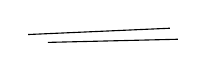
\begin{tikzpicture}\draw (0,0)--(1.8,0.08);\draw (0.25,-0.1)--(1.9,-0.06);\end{tikzpicture}}

Travaillons dans $\mathrm{DRstrat}(X)$. Notons que l'objet $\widetilde X$ de $\widetilde{\mathrm{DRst}}$ associé à $X$ couvre l'objet final (par définition des objets de $\mathrm{DRstrat}$). Donc on peut utiliser \deleted{$\mathrm{DRstrat}$} $\widetilde X$ pour écrire une suite spectrale de Leray
\[
H^*(X_{\mathrm{DRst}},O)\Longleftarrow E_2^{pq}=H^p(\unsure{\nu|\gamma}\longmapsto H^q(\widetilde X^{\unsure{\nu|\gamma}+1},O))
\]
\mspage{28}
